\documentclass{ximera}
\input{../preamble.tex}

\author{D. Davis \and R. Speckert \and N. Shay \and A. Davis}
\title{Need Title} \license{CC BY-NC-SA 4.0}
\begin{document}

\begin{abstract}
\end{abstract}
\maketitle

\begin{onlineOnly}
\section*{Need Title}
\end{onlineOnly}

\subsection*{Data Collection Activity}
\begin{center}
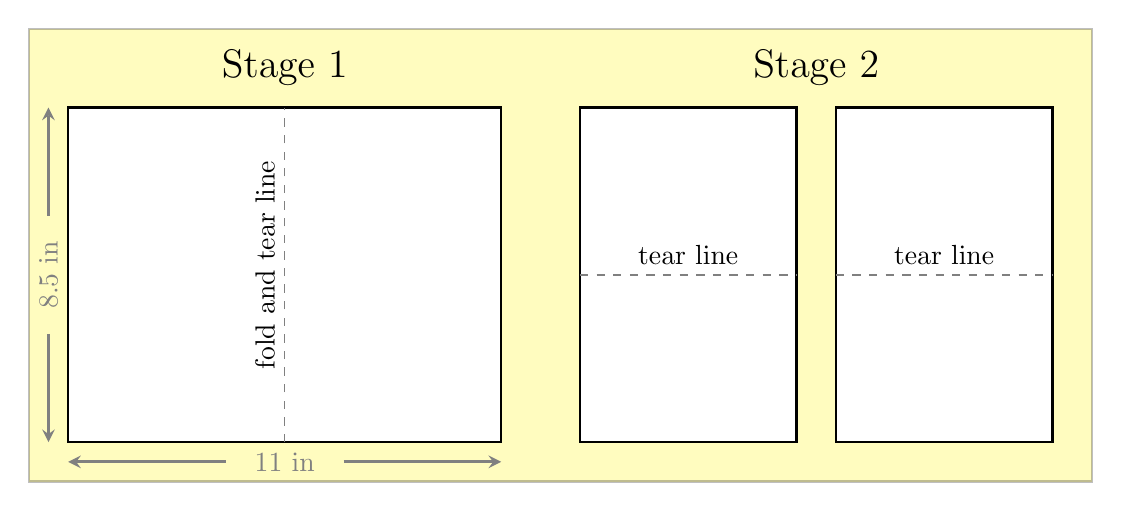
\begin{tikzpicture}[scale=0.5]
\draw[black, thick, fill=yellow,opacity=0.25] (-1,-1) rectangle (26, 10.5);
 \draw[black, thick, fill=white] (0,0) rectangle (11,8.5);
 \draw[line width=0.5pt, dashed, gray](5.5,0)--(5.5,8.5);
\node[rotate=90] at (5,4.5)   {fold and tear line};
\draw[line width=1pt,gray, stealth-](0,-0.5)--(4,-0.5);
\draw[line width=1pt,gray, -stealth](7,-0.5)--(11,-0.5);
\node[gray] at (5.5,-0.5)   {11 in};
\draw[line width=1pt,gray, -stealth](-0.5,2.75)--(-0.5,0);
\draw[line width=1pt,gray, -stealth](-0.5, 5.75)--(-0.5, 8.5);
\node[rotate=90, gray] at (-0.5,4.25)   {8.5 in};

\draw[black, thick, fill=white] (13,0) rectangle (18.5,8.5);
\draw[black, thick, fill=white] (19.5,0) rectangle (25,8.5);
 \draw[line width=0.5pt, dashed, gray](13,4.25)--(18.5,4.25);
  \draw[line width=0.5pt, dashed, gray](19.5,4.25)--(25,4.25);
 \node[] at (15.75,4.75)   {tear line};
  \node[] at (22.25,4.75)   {tear line};
%  \draw[line width=1pt,gray, stealth-](19.5,-0.5)--(21,-0.5);
% \draw[line width=1pt,gray, -stealth](23.75,-0.5)--(25,-0.5);

\node[] at (5.5,9.5)   {\Large{Stage 1}};
\node[] at (19,9.5)   {\Large{Stage 2}};
\end{tikzpicture}

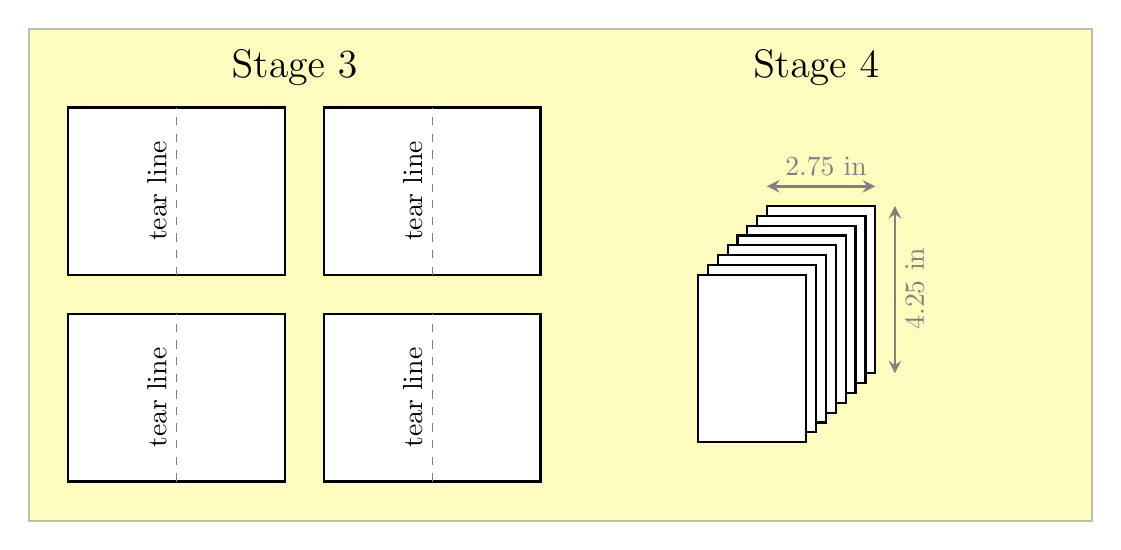
\begin{tikzpicture}[scale=0.5]
 \draw[black, thick, fill=yellow,opacity=0.25] (-1,-1) rectangle (26, 11.5);
 \draw[black, thick, fill=white] (0,0) rectangle (5.5, 4.25);
 \draw[black, thick, fill=white] (6.5,0) rectangle (12,4.25 );
  \draw[black, thick, fill=white] (0,5.25) rectangle (5.5, 9.5);
   \draw[black, thick, fill=white] (6.5,5.25) rectangle (12, 9.5);

  \draw[line width=0.5pt, dashed, gray](2.75,5.25)--(2.75,9.5);
\draw[line width=0.5pt, dashed, gray](2.75,0)--(2.75,4.25);
\draw[line width=0.5pt, dashed, gray](9.25,0)--(9.25,4.25);
\draw[line width=0.5pt, dashed, gray](9.25,5.25)--(9.25,9.5);
  
\node[rotate=90] at (2.25,2.13)   {tear line};
\node[rotate=90] at (2.25,7.38)   {tear line};
\node[rotate=90] at (8.75,2.13)   {tear line};
\node[rotate=90] at (8.75,7.38)   {tear line};

\draw[black, thick, fill=white] (17.75,2.75) rectangle (20.5, 7);
\draw[black, thick, fill=white] (17.5,2.5) rectangle (20.25, 6.75);
\draw[black, thick, fill=white] (17.25,2.25) rectangle (20, 6.5);
\draw[black, thick, fill=white] (17,2) rectangle (19.75, 6.25);
\draw[black, thick, fill=white] (16.75,1.75) rectangle (19.5, 6);
\draw[black, thick, fill=white] (16.5,1.5) rectangle (19.25, 5.75);
\draw[black, thick, fill=white] (16.25,1.25) rectangle (19, 5.5);
 \draw[black, thick, fill=white] (16,1) rectangle (18.75, 5.25);

 \draw[line width=1pt,gray, stealth-](17.75,7.5)--(19,7.5);
\draw[line width=1pt,gray, -stealth](19,7.5)--(20.5,7.5);
\node[gray] at (19.25,8)   {2.75 in};
\draw[line width=1pt,gray, stealth-](21,2.75)--(21,6);
\draw[line width=1pt,gray, -stealth](21, 6)--(21, 7);
\node[rotate=90, gray] at (21.5,4.9)   {4.25 in};

\node[] at (5.75,10.5)   {\Large{Stage 3}};
\node[] at (19,10.5)   {\Large{Stage 4}};
\end{tikzpicture}
\end{center}
At the end of the process you will have eight small rectangles, as shown in Stage 4.
\begin{question}
    Use the Pythagorean Theorem to complete the following expression for the length of the diagonal of the rectangle.  Then find the length of the diagonal to the nearest tenth of an inch.
    $$2.75^2+\answer{4.25}^2=d^2$$
    $$d=\answer{5.1}\,\text{in}$$
\end{question}

\begin{question}
    You will be using centimeter rulers to measure the diagonals of the rectangles.  Let's convert the theoretical length of the diagonal to centimeters.  Use the 
    \end{question}

\begin{onlineOnly}
\begin{center} 
\geogebra{ajtk6jux}{950}{600} 
\end{center}
\end{onlineOnly}

\section*{Practice Problems}

\section*{References}
Wafer photo credit: \textit{Processed 200 mm Si Wafer} by Goldenvu CC BY-SA 4.0.

\end{document} 